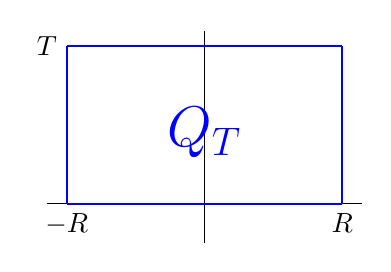
\begin{tikzpicture}

\draw (-2, 0) -- (2, 0);
\draw (0, -0.5) -- (0, 2.2);

\draw[blue, thick] (1.75, 0) -- (1.75, 2);
\draw[blue, thick] (-1.75, 0) -- (-1.75, 2);

\node[below] at (-1.75, 0) {$-R$};
\node[below] at (1.75, 0) {$R$};
\node[left] at (-1.75, 2) {$T$};


\draw[blue, thick] (-1.75, 0) -- (1.75, 0);
\draw[blue, thick] (-1.75, 2) -- (1.75, 2);

\node[blue] at (0, 0.9) {\huge $Q_T$};

\end{tikzpicture}